\section{Block-based Symmetry Breaking}
\label{sec::blocks2}

The idea we develop in this section 
is to localise straight-move jump points with bitwise operations.  
This implementation allows to manipulate 
many nodes rapidly, 
improving the overall runtime.  

\begin{figure}[ht]
  \begin{center}
    \scalebox{0.8}{%
      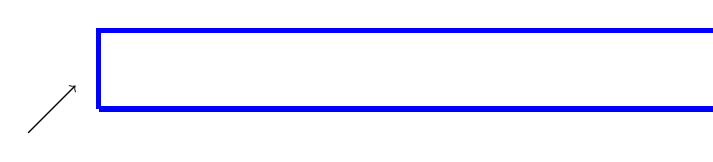
\begin{tikzpicture}
        \creategrid{10}{3}
        \drawobstacle{4}{1}
        \drawobstacle{5}{1}
        \drawobstacle{7}{2}
%        \drawobstacle{7}{4}
%        \drawobstacle{6}{4}
%        \drawobstacle{3}{7}
%        \drawobstacle{2}{2}
%        \drawobstacle{3}{2}
        \draw[->] (0.7,0.7) -- (1.3,1.3);
        \drawgridnode{2}{2}{$N$}
        \drawgridnode{1}{1}{$P$}
%        \drawgridnode{7}{5}{$Z$}
        \drawgridnode{3}{2}{{\color{red} 1}}
        \drawgridnode{2}{1}{{\color{red} 2}}
        \drawgridnode{2}{3}{{\color{red} 3}}
        \drawgridnode{4}{2}{{\color{red} 4}}
        \drawgridnode{3}{1}{{\color{red} 5}}
        \drawgridnode{3}{3}{{\color{red} 6}}
        \drawgridnode{5}{2}{{\color{red} 7}}
        \drawgridnode{4}{1}{{\color{red} 8}}
        \drawgridnode{4}{3}{{\color{red} 9}}
        \draw[blue,line width=2pt] (1,1) -- (9,1) -- (9,2) -- (1,2) -- (1,1);
      \end{tikzpicture}%
    }
  \end{center}
  \caption{A current search state 
    (the grid is assumed larger than the part presented).
  The red numbers show in which order the traversability of the nodes 
  is tested.}
  \label{fig::gridforblocks}
\end{figure}

Consider the grid presented on Figure~\ref{fig::gridforblocks} 
(this is supposed to be a small chunk of a larger grid).  
The node currently being explored is $N = \langle 2,2\rangle$ 
and its parent is $P = \langle 1,1\rangle$.  
At this stage, the horizontal and vertical axes must be scanned 
for jump point before another diagonal move is taken.  
As it turns out, a jump point will be found in $\langle 6,2\rangle$.  
When looking for a jump point on row $2$, 
the status (traversable or not) of the nodes 
will be checked more or less in the order given by the numbers in red, 
depending on the actual implementation.  
Each one of these nodes will be individually tested.  

Because each node is represented by a single bit, 
it is possible to manipulate large blocks of data.  
The status of the eight nodes in the blue rectangle 
starting from $\langle x,y\rangle = \langle 2,2\rangle$ in the figure 
could for instance be represented by a single byte $B$ 
whereby the $i$th bit $B[i]$ of the byte is set to $1$ 
iff the node $\langle x+i,y\rangle$ of the grid contains an obstacle.  
(Practically, we use 32-bit words in the implementation, 
but this discussion will stick with 8-bit bytes for simplicity.)
In particular, it would be easy to see that the block 
between $\langle 2,3\rangle$ and $\langle 9,3\rangle$ 
is obstacle-free because the corresponding byte evaluates to $0$.  

More generally, we can build a byte 
which will represent the list of positions 
at which the agent must stop.  
If this byte evaluates to $0$, 
we can jump $7$ steps (here, to $\langle 9,2\rangle$) 
and keep searching for the next $8$ cells.  
There are three reasons why the agent may have to stop: 
a cell with a forced neighbour (above or below) was found 
or an obstacle was reached.  
A byte $B_S$ is computed for each reason 
and they are merged with a byte-wise or.  
A forced neighbour exists in position $i$ 
if there is an obstacle at position $i-1$ 
and no obstacle at position $i$; 
this is computed with the byte-wise operations \texttt{(B>>1\ \& !B)}.  
For instance on row $1$, $B_{\mathrm{below}} = [0,0,1,1,0,0,0,0]$ 
which leads to 
$\mathit{forced\_neighbour}(B_{\mathrm{below}}) = [0,0,0,0,1,0,0,0]$.  
The byte that represents the current row already indicates 
where the obstacles are.  
In the example of the figure, 
we obtain the byte $B_S = 
\mathit{forced\_neighbour}(B_{\mathrm{below}})\ |\ 
\mathit{forced\_neighbour}(B_{\mathrm{above}})\ |\ 
B_{\mathrm{current}}
= [0,0,0,0,1,1,0,0]$.  
Because $B_S \neq 0$, 
we know that the search has to stop.  
We use the C \texttt{ffs} command 
to extract the position of the first $1$ 
and determine the position where to jump to.  
Since this position contains no obstacle, 
it is a jump point; 
otherwise, there would be no jump point on the row.  

Naturally, a copy of the map is made to account for vertical scans.  
Furthermore, the algorithm must be slightly adapted 
for cases where the direction of travel is right-to-left 
instead of left-to-right.  



%EOF 
